\chapter{Related Work}{}
\label{sec:related}

\lettrine[lraise=0.1, nindent=0em, slope=-.5em]{S} {NIPR IS RELATED TO} prior work in three areas: tailoring search interfaces for specific tasks; example-centric programming; and systems for making code more suited to a given context.

\fancybreak{\pfbreakdisplay}

\section{Search Interfaces}
\label{sec:searchengines}

Nowadays, search interfaces are supporting a range of specific tasks~\cite{Brandt:2009jb, Morville:2010up, Wightman:2012gc}, from Web task automation to programming. For Web automation~\cite{Little:2007dh, Miller:2008ge, Cypher:2010ub}, search interfaces allow users to write scripts in the most simple and natural way, like `now click the search button', and the search interface will interpret this input by searching an API that will make sense of this input. For programming, search interfaces allow programmers to query code repositories to find keyword and structural matches~\cite{Mandelin:2005uj, Bajracharya:2006vn, Sahavechaphan:2006tc, Bajracharya:2010um}. With keyword matches, the search is limited to text analysis (no code semantics), while with structural matches, the search has a bigger scope. That is, with structural search, the search interface can determine how the code works---via static analysis or via test cases~\cite{Hummel:eq, LazzariniLemos:2007jh, Reiss:2009fu}---and respond to a query more appropriately. For example, searching for a snippet that computes the anagram of the word ``anaconda.'' 

Undeniably, these types of search interfaces have improved how developers locate code snippets. Large sets of code snippets (i.e., example code) are just one search away. Clearly, this easy access to such an amazing treasure trove code has a value; however, it also has significant limitations. Besides the inability to effectively locate general code structures(Keyword matches), or to assist in searching for snippets even when the developers don't know the names of relevant modules (methods that implement an API), or types, these interfaces are less effective in justifying the suitability of found code. With regard to how current programming search interfaces differ from \uppercase{SnipR}, it is envisioned that \uppercase{SnipR} is not seen as their competitor, but more like a platform: a platform for searching for suitable code via code retargeting.
% 
% 
% In recent years many code-centric search engines have appeared. These engines rely on either keywords, unit tests, open source project's metadata, semantic information, or any combination thereof to find large sets of relevant example code. Undeniably, these engines have changed how developers find information. Large sets of example code are just one search away. This easy access to such an amazing treasure of trove code clearly has value; however, it has also significant limitations as a platform. These engines leave the suitability scrutiny---done manually---of returned results to the developers. With regard to how these engines differ from \uppercase{SnipR}, it is envisioned that \uppercase{SnipR} is not seen as a competitor to any code search search engine, but more like a platform: a platform these engines can use for finding suitable example via code retargeting.
% % These engines utilize sophisticated ranking formulas for returning results that correspond with the developers' search, leaving the suitability scrutiny---done manually---of returned results to the developers.
 
\fancybreak{\pfbreakdisplay}

\section{Recommending Suitable Examples}
\label{sec:codesearch}

Many systems have been built to help developers find trustable and relevant example code, including systems that have leveraged crowdsourced input to suggest solutions to developers' code problems. Broadly speaking, \uppercase{SnipR} differs from this prior work by supporting a direct exploration of potential future code changes of found examples (Figure~\ref{fig:basealternative}). Providing this sort of direct exploration can increase the code search's effectiveness, efficiency, and user satisfaction. Not only the developer can get expose to many variations of the same code, but also the developer can have more confidence sooner that the picked examples are the right ones. Consequently, the developer could avoid some of the ``round-trip'' errors that can arise when developers iteratively edit unsuitable example code.

\begin{figure}[!ht]
    \centering
    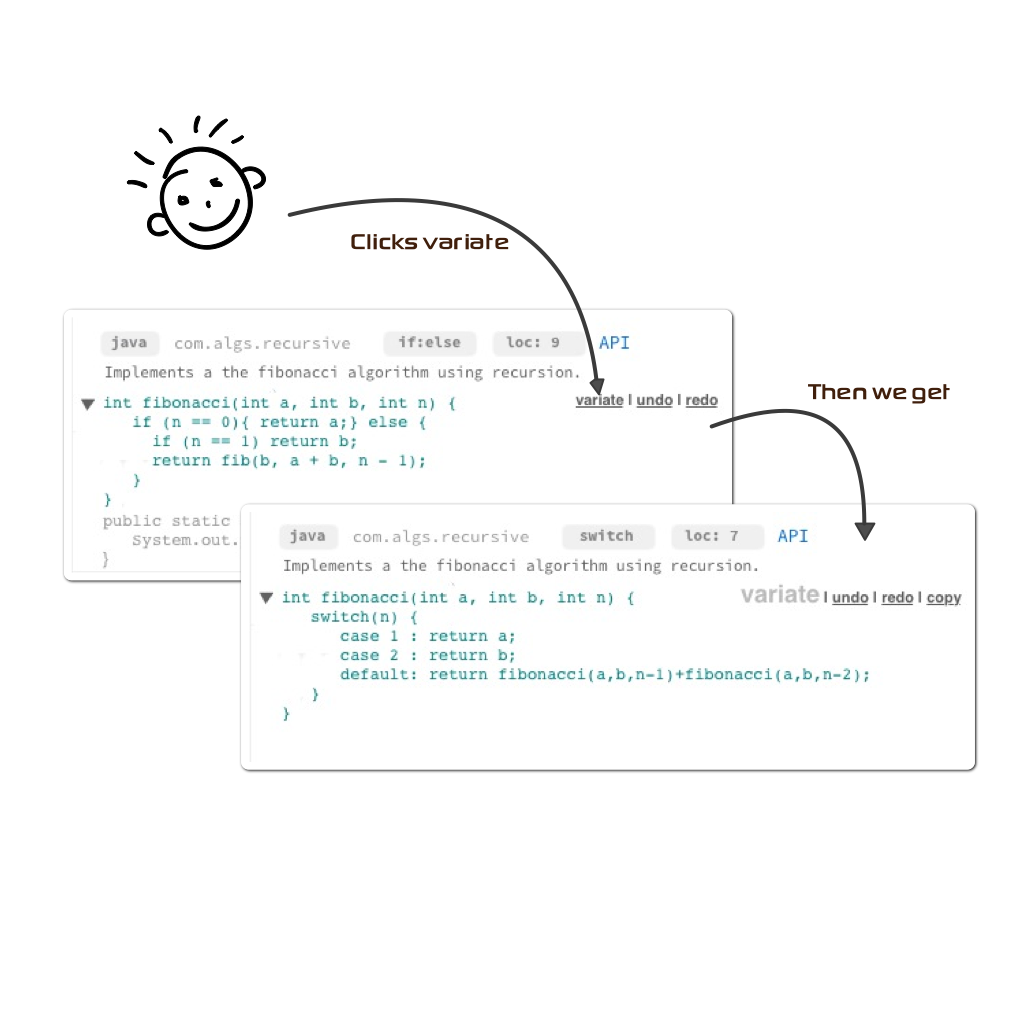
\includegraphics[width=\textwidth]{images/basealternative}
    \caption{Exploration of potential future code changes of a single result.}
    \label{fig:basealternative}
\end{figure}
% \pagebreak

For example, Hartmann's HelpMeOut system~\cite{Hartmann:2010hx} aids the debugging of code-related error messages by suggesting solutions that peers have applied in the past. McMillan's Source Code Recommender systems~\cite{McMillan:2012dj} combines mining written code specifications and open sourced code to recommend source code modules relevant to the application under development. Gysin's solution~\cite{Gysin:2010kt} uses a trustability metric based on developers' karma to find and recommend trustable code. EUKLAS\footnote{\url{http://www.cs.cmu.edu/~euklas}} highlights simple source code errors and suggest the appropriate corrections. Lastly, Stolee's semantic search approach~\cite{Stolee:2012wp} uses lightweight specifications and a SMT solver to deal with the search of suitable code.  

% dont trust me just because I am telling u to do it. E.g., dont trust this code is relevant just because there is a score that tells u that.

\fancybreak{\pfbreakdisplay}

\section{Retargeting Source Code}
\label{sec:retargetingcode}

Adapting a code example to a different context is tedious and difficult. Partly because there are many different types of code modifications that might be required to make this code more suited---e.g., variables renamed, and dependencies included. Various attempts have been made to address this problem, many of them include systems for resolving many simple coding errors, systems for suggesting ways for correcting compiler and runtime errors, systems for end-user modification of web experiences, or systems for making incremental code changes to available example code in order to make it more suited. Unlike \uppercase{SnipR}, any interaction for modifying any code example is done directly in the IDE or in a visual web-based development environment.  

Wightman's SnipMatch~\cite{Wightman:2012gc} introduces a markup that allows snippet authors to specify search patterns and integration instructions. SnipMatch uses this information---in conjunction with the current code context and the willingness to curate and share snippets---to semi-automate the integration of a code example. Nita's Twinning~\cite{Nita:2010en} allow programmers to specify a set of code-level mappings between alternative APIs. With Twinning, programmers can specify changes that modify a program from using one API to using an alternative API. Similarly to SnipMatch, Twinning is also dependent on developers' willingness to define mappings by hand. In such a case, the developers need to manually express all the correspondences between two programs, apply the mapping to a program, compile the program, and then rely on type errors to identify the next course of action.  Similar systems include the Eclipse QuickFix and Ernst's Quick Fix Scout\footnote{\url{https://code.google.com/p/quick-fix-scout/}}. These tools allow programmers to quickly resolve many simple errors. Oney's Codelets~\cite{Oney:2012ge} system allows authors of example code to use a form of markup language to indicate those code's regions that can be edited. Lastly, Hartmann's d.mix~\cite{Hartmann:2007wf} allow a direct experimentation of found code on the Web.

Of the above prior work, SnipMatch and Twinning are the most similar to \uppercase{SnipR}---at least on the surface. SnipMatch shares with \uppercase{SnipR} the use of instructions for changing code snippets, sloppy interpretation of keyword commands into some executable code, and the social-software mechanism of sharing scripts. Twinning shares with \uppercase{SnipR} the use of an abstract syntax for representing mapping-based program transformations. \uppercase{SnipR} distinguishes itself in two important ways. First, SnipMatch and Twinning are technologies that require an ongoing manual effort associated with creating and modifying source code templates and mapping-based transformations. The success of these tools is dependent on whether a template or mapping has already been created by a developer. \uppercase{SnipR} is more akin to an automatic approach for learning mapping-based transformations from code examples at a larger scale (See Chapter~\ref{chap:algorithms} for more details) via a machine learner. Second, SnipMatch and Twinning were designed to work in an offline setting, such as a plugin in an IDE (SnipMatch), and as a component in the Cornell Polyglot source-source translation framework\footnote{\url{http://www.cs.cornell.edu/projects/polyglot}}. In contrast, with \uppercase{SnipR} developers will use their Web browser for doing code retargeting. Third, \uppercase{SnipR} differs from these tools in focus and approach. \uppercase{SnipR} focuses on helping developers justify the suitability of code examples during their search-driven development activities by applying retargeting operations (See Chapter~\ref{chap:twist} for details on how retargeting operations are invoked). The other two focus on either specifying and applying a class of program transformation (and storing them long-term), or creating code integration templates which will assist developers in integrating a snippet into their projects.  
